\chapter[Introdução]{Introdução}

A utilização de agentes de software constitui uma abordagem adequada para a concepção e a construção de sistemas complexos e distribuídos \cite{silva2003padroes}. Tais agentes conhecem os interesses dos usuários e podem agir de forma autônoma em prol dos mesmos. Ao invés de exercer controle completo, o papel dos usuários dá-se, preferencialmente, de forma cooperativa com os agentes de software, de modo que esses últimos possam auxiliar esses usuários no cumprimento de suas metas \cite{green1997}.

Agentes de software despertam o interesse de diversos pesquisadores e empresas de software \cite{green1997}. Trata-se de uma área que está emergindo rapidamente dentro da TI \cite{jennings1996}, como um paradigma poderoso para projetar e desenvolver sistemas de software complexos \cite{zambonelli2001}. 

%Outro fator ressaltado pelo autor é forma dinâmica e não estruturada com que informações são geradas.%

Sistemas Multiagentes (SMA) encontram espaço em uma série de domínios de aplicação, como: comércio eletrônico, \textit{design} de interface, jogos e gestão de processos industriais e comerciais complexos \cite{jennings1996}. \citeonline{green1997} apontam outras áreas de aplicação como controle de tráfego aéreo, \textit{data mining}, recuperação e gestão da informação, educação e assistentes digitais pessoais (\textit{Personal Digital Assistants}, PDAs).

Uma das armadilhas apontadas por \citeonline[pág. 246]{livrao} ocorre quando agentes interagem muito livremente ou de forma desorganizada. A dinâmica de SMA é complexa e, portanto, pode se tornar caótica. Para descobrir o que acontecerá em seguida no sistema, muitas vezes, é necessário executar o sistema repetidamente. O número de agentes também influencia em termos de complexidade para gerir de forma eficaz o sistema. 

Independentemente do paradigma adotado, é habitual que desenvolvedores comecem a codificar sem uma arquitetura formal clara e bem definida \cite{richards2015software}. O resultado desta prática, frequentemente, é uma coleção de módulos de código-fonte desorganizados, que não possuem papéis, responsabilidades e relacionamentos claros uns com os outros. 

Segundo \citeonline{richards2015software}, aplicações que não possuem uma arquitetura formal são geralmente ``acopladas, quebradiças, difíceis de mudar e sem uma visão ou direção clara". Questões básicas sobre implantação, manutenção e escalabilidade desses sistemas são difíceis de definir. 

Uma alternativa é adotar padrões arquiteturais. Estes ajudam a definir as características básicas e o comportamento de uma aplicação \cite{richards2015software}. O arquiteto de software deve conhecer as características, pontos fortes e fracos de cada padrão arquitetural, afim de optar por aquele que atenda às suas necessidades e aos seus objetivos comerciais específicos. 

%Por exemplo, alguns padrões de arquitetura naturalmente se prestam a aplicações altamente escaláveis, enquanto outros padrões de arquitetura naturalmente se prestam a aplicações que são altamente ágeis.%


%%%%%%


De acordo com \citeonline{shaw1996}, descrições uniformes das arquiteturas, quando disponíveis, são instrumentos para simplificar esta escolha. Segundo \citeonline{avgeriou2005}, o processo de descrever, encontrar e aplicar padrões arquiteturais na prática ainda é largamente \textit{ad-hoc} e não sistemático. Isto se deve a várias questões que ainda não foram resolvidas como, por exemplo, em relação à classificação ou catalogação de padrões que podem ser usados por arquitetos de software.

%%%%%

Cabe destacar que existe um paralelo entre a complexidade das organizações e os SMA. Organizações são entidades complexas formadas para superar várias limitações de instâncias individuais, tais como limitações cognitivas, físicas, temporais e institucionais \cite{van2004organizational}. Neste sentido, são utilizados conceitos, métodos e técnicas de \textit{design} organizacional humano como princípios arquitetônicos para SMA \cite{van2004organizational}. 

%a arquitetura de um SMA pode, naturalmente ser vista como uma organização computacional \cite{zambonelli2001}. o \textit{design} e análise de tais sistemas podem basear-se em abstrações organizacionais \cite{zambonelli2001}. % 

Uma organização fornece uma estrutura para as interações dos agentes através da definição de papéis, expectativas de comportamento e relações de autoridade \cite{sycara1998multiagent}. As organizações são, em geral, conceitualizadas em termos de sua estrutura, isto é, o padrão de informações e relações de controle que existem entre os agentes e a distribuição das capacidades de resolução de problemas entre eles \cite{sycara1998multiagent}. 

Na resolução cooperativa de problemas, por exemplo, uma estrutura fornece a cada agente uma visão de alto nível de como o grupo soluciona problemas \cite{sycara1998multiagent}. Portanto, a estrutura organizacional impõe restrições sobre as formas como os agentes se comunicam e se coordenam. Neste contexto, os padrões arquiteturais para SMA baseados em estruturas organizacionais, podem fornecer soluções práticas para o desenvolvimento de SMA complexos, sendo assim, são objetos de estudo deste trabalho.

O catálogo a seguir baseia-se no trabalho de \citeonline{Argente200655} entitulado \textit{Multi-Agent System Development Based on Organizations}, bem como em outros estudos realizados e conhecimentos adquiridos pela autora dessa monografia junto à massa de artigos investigados e apresentados na Seção anterior. A Figura \ref{fig:my_patterns} representa as classificações de cada padrão dentro de categorias e subcategorias definidas, principalmente, pelos autores do referido artigo.



\begin{figure}[H]
    \centering
    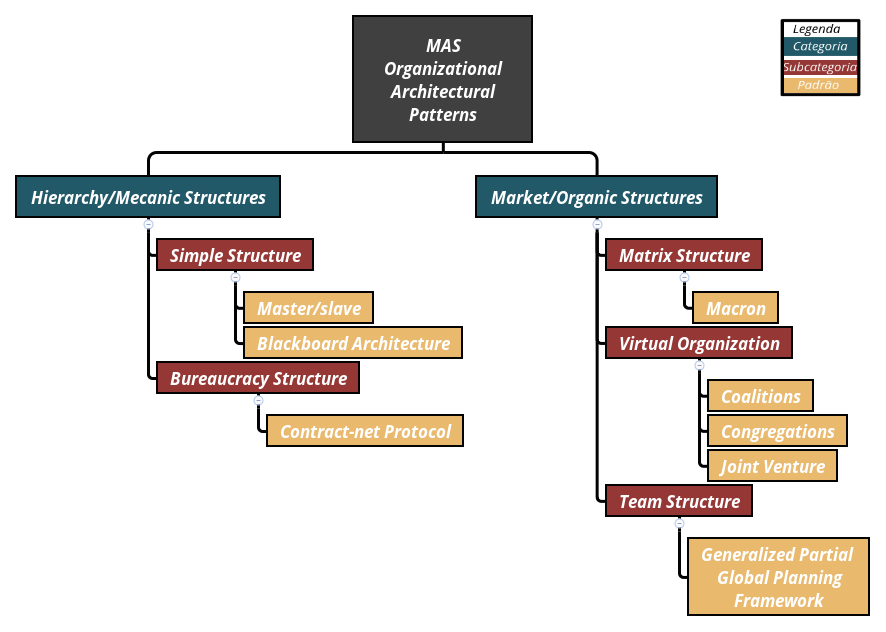
\includegraphics[scale=0.47]{figuras/mas_patterns.png}
    \caption{\textit{MAS - Organizational Architectural Patterns}. Fonte: Autora. Adaptado de: \citeonline{Argente200655}.}
    \label{fig:my_patterns}
\end{figure}










